\documentclass[11pt, oneside]{article} 
\usepackage{geometry}
\geometry{letterpaper} 
\usepackage{graphicx}
	
\usepackage{amssymb}
\usepackage{amsmath}
\usepackage{parskip}
\usepackage{color}
\usepackage{hyperref}

\graphicspath{{/Users/telliott_admin/Tex/png/}}
% \begin{center} 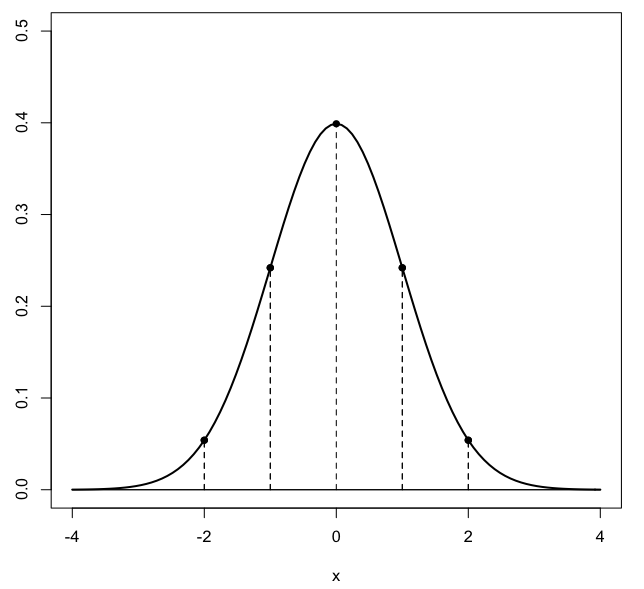
\includegraphics [scale=0.4] {gauss3.png} \end{center}

%break
\title{Cramer's rule}
\date{}

\begin{document}
\maketitle
\Large

This is a simple description of determinants in linear algebra and their uses.  Let's start with this example 
\[
\begin{bmatrix} 
  a  &  b \\ 
  c  &  d 
\end{bmatrix}
\]
The determinant of this matrix is $ad - bc$.  For a matrix A, we would indicate the determinant by writing $det(A)$ or by showing the matrix with straight vertical bars like this:
\[
\begin{vmatrix} 
  a  &  b \\ 
  c  &  d 
\end{vmatrix}
\]
For a 3 x 3 matrix like
\[
\begin{bmatrix} 
  a  &  b  &  c  \\ 
  d  &  e  &  f   \\
  g  &  h  &  i
\end{bmatrix}
\]
the determinant has three terms (or six, depending on how you count).  Some people like to remember it this way
\begin{center} 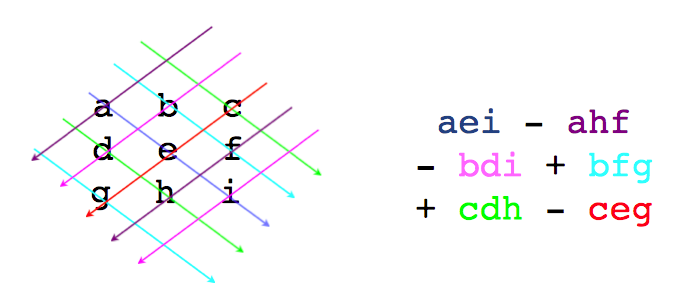
\includegraphics [scale=0.4] {dets_color.png} \end{center}
But this only works for $3 \times 3$.  The systematic way is to find the three terms by a standard rule, and use the "checkerboard."
The first term of three is
\[ a \ 
\begin{vmatrix} 
  e  &  f \\ 
  h  &  i 
\end{vmatrix}
\]
In other words, this term is equal to $a(ei - fh)$.  The entire determinant is
\[ a \ 
\begin{vmatrix} 
  e  &  f \\ 
  h  &  i 
\end{vmatrix}
-
b \ 
\begin{vmatrix} 
  d  &  f \\ 
  g  &  i 
\end{vmatrix}
+
c \ 
\begin{vmatrix} 
  d  &  e \\ 
  g  &  h 
\end{vmatrix}
\]
Written out on one line it is
\[ a(ei - fh) - b(di - fg) + c(dh-eg) \]
A key point about this calculation is the minus sign for the second term.  If we replace the matrix by a "checkerboard" of plus and minus signs
\[
\begin{bmatrix} 
  +  &  -  &  +  \\ 
  -  &  + &  -   \\
  +  &  -  &  +
\end{bmatrix}
\]
the term starting with b has a minus sign because that position in the checkerboard is $-$.  

The reason for bringing the checkerboard into it is that any row or column can be used to group what are called the "minors", the little 2 x 2 matrices.  The way that we did it above is shown in the top panel of the figure

\begin{center} 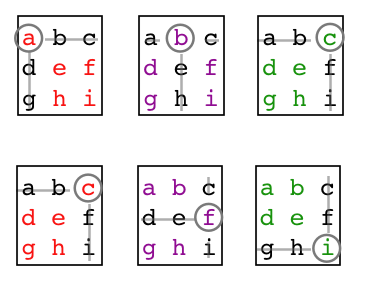
\includegraphics [scale=0.5] {det_detail.png} \end{center}

In the first row, we picked $a$ and then crossed out the rest of its row and column.  What is left is the "minor" for $a$ and we do
\[ a \ 
\begin{vmatrix} 
  e  &  f \\ 
  h  &  i 
\end{vmatrix}
\]
As described, in the end we get three cofactors ($a,b,c$) together with their minors, and the sign is determined by the checkerboard.  However, as an alternative, we might have chosen column 3 as shown in the bottom panel.  Then we'd have
\[ c \ 
\begin{vmatrix} 
  d  &  e \\ 
  g  &  h 
\end{vmatrix}
-
f \ 
\begin{vmatrix} 
  a  &  b \\ 
  g  &  h 
\end{vmatrix}
+
i \ 
\begin{vmatrix} 
  a  &  b \\ 
  d  &  e 
\end{vmatrix}
\]
Notice that the sign of each term follows the checkerboard rule.

Remember this rule!  It can be very useful if we have a matrix with some zeros in it like

\begin{center} 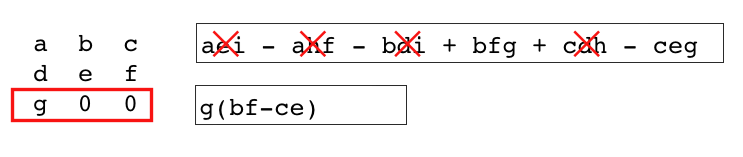
\includegraphics [scale=0.5] {det_crossout.png} \end{center}
We find the determinant of this matrix using the third row, it is just $g(bf-ce)$.  

The rule that any column or row can be the starting point to get the determinant can be proven correct by simple algebra.

It's not so important, but note that the formula for the determinant of a 2 x 2 matrix also follows the checkerboard rule.  $ad-bi$ is really $a \ det(d) - b \ det(c)$, with signs from the rule.

In Strang's Linear Algebra, he shows how the properties of the determinant follow from three basic rules.
\vspace{2 mm}

1.  The determinant of an $n$ x $n$ identity matrix is 1.
\vspace{2 mm}

\[
\begin{vmatrix} 
  1  &  0 \\ 
  0  &  1 
\end{vmatrix}
= 1
\]

2.  The determinant changes sign with a row exchange.
\vspace{2 mm}

\[
\begin{vmatrix} 
  0  &  1 \\ 
  1  &  0 
\end{vmatrix}
= -1
\]

3.  The determinant is a linear function of each row separately.
\vspace{2 mm}

\[
\begin{vmatrix} 
  ta  &  tb \\ 
  c  &  d 
\end{vmatrix}
= t
\begin{vmatrix} 
  a  &  b \\ 
  c  &  d 
\end{vmatrix}
\]
\[
\begin{vmatrix} 
  2  &  1 \\ 
  1  &  2 
\end{vmatrix}
= 3, \ \ 
\begin{vmatrix} 
  4  &  2 \\ 
  1  &  2 
\end{vmatrix}
= 6, \ \ 
\begin{vmatrix} 
  4  &  2 \\ 
  2  &  4 
\end{vmatrix}
= 12
\]

However, it is the fourth rule (that follows from these three) that is crucial:
\vspace{2 mm}

4.  If two rows of a matrix are identical, then $det(A) = 0$.
\vspace{2 mm}
\[
\begin{vmatrix} 
  1  &  2 \\ 
  1  &  2 
\end{vmatrix}
= 0
\]
The converse is also true.  If we set up a matrix to solve a system of equations, and the determinant of that matrix is 0, there is not a unique solution.  This means, for example that 
\[
\begin{vmatrix} 
  ta  &  tb \\ 
  a  &  b 
\end{vmatrix} = 0
\]
as you can easily see by subtracting t times the second row from the first.  You obtain a row of zeros, and as we showed above, any matrix with a row (or column) of zeros has a determinant equal to 0.

Cramer's Rule is a rule for solving systems of equations that relies on determinants.  It's very popular with high school math teachers because it leads to problems with lots of arithmetic, where you may make a mistake!

Suppose we have a 2 x 2 system with equations that we arrange in this form
\[ ax + by = p \]
\[ cx + dy = q \]
We arrange the coefficients of x and y in a matrix and calculate its determinant
\[ D = 
\begin{vmatrix} 
  a  &  b \\ 
  c  &  d 
\end{vmatrix} = ad - bc 
\]
Next we construct two more matrices and calculate their determinants.  The first one is constructed by replacing the "x" column with p and q
\[ D_x = 
\begin{vmatrix} 
  p  &  b \\ 
  q  &  d 
\end{vmatrix} = pd - bq 
\]
The second one replaces the "y" column with p and q
\[ D_y = 
\begin{vmatrix} 
  a  &  p \\ 
  c  &  q 
\end{vmatrix} = aq - cp 
\]
The solutions are 
\[ x = \frac{D_x}{D}, \ \ \ \ 
y = \frac{D_y}{D} \]
Notice how the requirement that the determinant of the coefficients matrix cannot be equal to zero shows up in this method.  We can't divide by zero, so the first determinant $D$ cannot be equal to 0.

For 3 x 3 it is the same approach, just the arithmetic is longer.
\[ ax + by + cz = p \]
\[ dx + ey + fz = q \]
\[ gx + hy + iz = r \]

\[ D = 
\begin{vmatrix} 
  a  &  b  &  c  \\ 
  d  &  e  &  f   \\
  g  &  h  &  i
\end{vmatrix}, \ \ \ \ 
D_x = 
\begin{vmatrix} 
  p  &  b  &  c  \\ 
  q  &  e  &  f   \\
  r  &  h  &  i
\end{vmatrix},   \ \ \ \
D_y = 
\begin{vmatrix} 
  a  &  p  &  c  \\ 
  d  &  q  &  f   \\
  g  &  r  &  i
\end{vmatrix},  \ \ \ \ 
D_z = 
\begin{vmatrix}
  a  &  b  &  p  \\ 
  d  &  e  &  q   \\
  g  &  h  &  r
\end{vmatrix} 
\]
The solutions are 
\[ x = \frac{D_x}{D}, \ \ \ \ 
y = \frac{D_y}{D} , \ \ \ \
z = \frac{D_z}{D} \]
It is easy enough to derive Cramer's rule.  Let's do it for 2 x 2.  Suppose we have
\[ ax + by = p \]
\[ cx + dy = q \]
Solve eqn 1 for $x$ and substitute the result into eqn 2
\[ x = \frac{p - by}{a} \]
\[ c (\frac{p - by}{a}) + dy = q \]
\[ cp - cby + ady = aq \]
\[ y = \frac{aq-pc}{ad-bc} = \frac{D_y}{D} \]
Or solve eqn 1 for $y$ and substitute the result into eqn 2
\[ y = \frac{p - ax}{b} \]
\[ cx + d(\frac{p - ax}{b}) = q \]
\[ bcx + dp - adx = bq \]
\[ x = \frac{bq-dp}{bc-ad} = \frac{dp-bq}{ad-bc} = \frac{D_x}{D} \]


A bit more complicated, but this also works.  Take the first result, the value for y, and substitute into the eqn for x above
\[ x = \frac{1}{a} (p - by) = \frac{1}{a} [p - b(\frac{aq-pc}{ad-bc} )]                     \]
Multiply $p$ by $(ad-bc)$ on top and bottom to get a common denominator
\[ \frac{1}{a} [p \frac{(ad-bc)}{(ad-bc)} - b(\frac{aq-pc}{ad-bc} )]   \]
Simplifying the numerator
\[ (\frac{1}{ad-bc}) (\frac{pda}{a} - \frac{pbc}{a} - \frac{baq}{a} + \frac{bpc}{a} ) =  \frac{pd - bq}{ad-bc} =  D_x  \]



\end{document}  